%
% Copyright (c) 2017  Zubax Robotics OU  <info@zubax.com>
%
% Distributed under BY-NC-ND (attribution required, non-commercial use only, no derivatives).
%

\documentclass{zubaxdoc}
\graphicspath{{document_templates/documentation_template_latex/}}

\title{Zubax Orel 20 Datasheet}

\begin{document}
\frontmatter

\begin{titlepage}

\section*{Overview}

Zubax Orel 20 is an advanced sensorless BLDC propeller drive controller with doubly redundant CAN bus interface.
Zubax Orel 20 runs the Sapog\footnote{Refer to the Sapog Reference Manual for information.}
firmware.

\section*{Features}

\begin{itemize}
    \item Excellent dynamic characteristics.
    \item Regenerative braking and active freewheeling.
    \item 350 W continuous power output at 10 g weight.
    \item Optional RPM control loop (RPM governor).
    \item Self diagnostics and health status reporting.
    \item Highly configurable.
    \item Low noise and low current ripple due to low ESR embedded filtering capacitors and high frequency PWM.
    \item Supported interfaces:
    \begin{itemize}
        \item CAN, with optional double redundancy.
        \item UART.
        \item RCPWM (analog PWM interface widely used in robotics).
    \end{itemize}
    \item High quality assurance:
    \begin{itemize}
        \item Every manufactured unit undergoes a strict testing procedure.
        The testing log for each produced unit is available to the user via the website at\\
        \url{https://device.zubax.com/device_info}.
        \item Protection against unlicensed (counterfeit) production by means of a digital signature
        installed on every manufactured unit.
    \end{itemize}
    \item Open source firmware -- Sapog (3-clause BSD license).
\end{itemize}

\BeginRightColumn
\section*{Applications}

\begin{itemize}
    \item Propeller drives for unmanned aerial vehicles.
    \item Pump and propeller drives for unmanned watercraft.
\end{itemize}

\centering
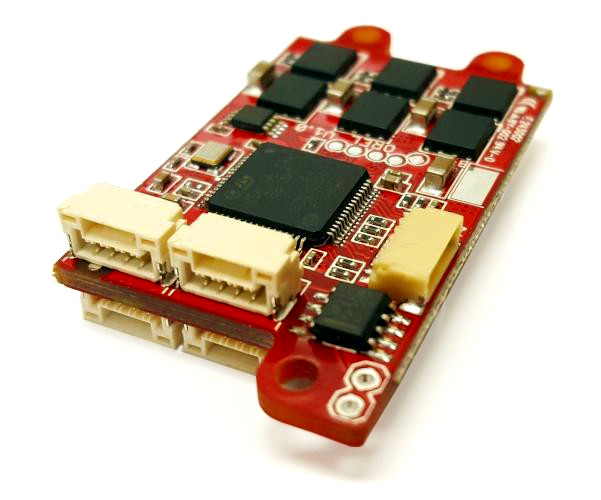
\includegraphics[width=0.45\textwidth]{image}
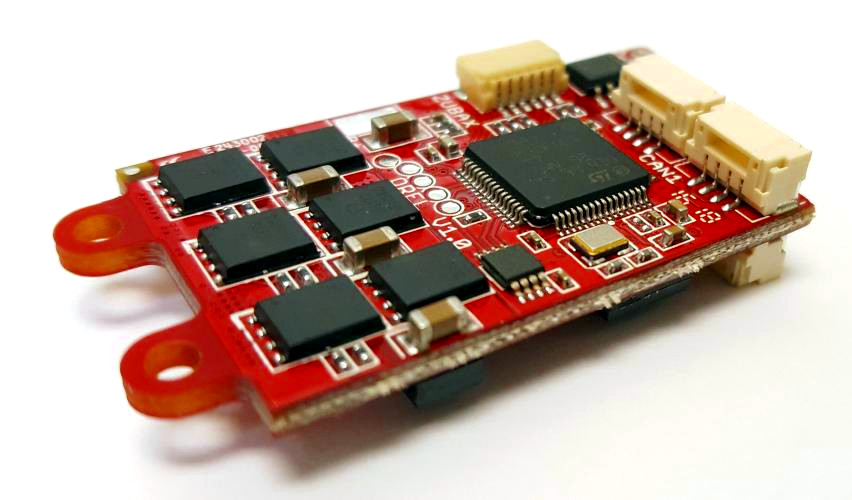
\includegraphics[width=0.45\textwidth]{image2}
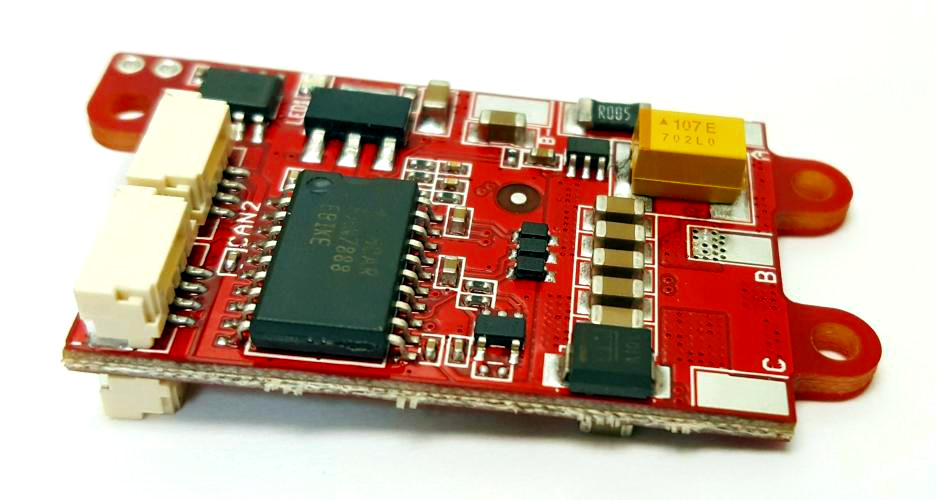
\includegraphics[width=0.45\textwidth]{bottom}

\end{titlepage}

\tableofcontents
\listoffigures
\listoftables

\mainmatter

\chapter{Overview}

Zubax Orel 20 is an advanced controller of sensorless BLDC motors designed for use in
cost sensitive applications.
Its primary application domains include propulsion systems of electric unmanned aircraft
and watercraft.

Zubax Orel 20 runs Sapog - an open source multiplatform BLDC controller firmware
developed by Zubax Robotics.
Please refer to the Sapog Reference Manual\footnote{Available from the Zubax Robotics website.}
for its usage information.
This datasheet is focused only on the hardware aspect of the product.

\section{System integration}

Zubax Orel 20 is a single supply device, which means that the device does
not require any supply inputs except for the high power supply.
The 5 V rails of the CAN interfaces are not used by the device; rather,
they connect the 5 V rails of their respective CAN connector pairs directly together.

Application-specific integration documentation is available on the Zubax Robotics website.

\begin{figure}[hb]
    \centering
	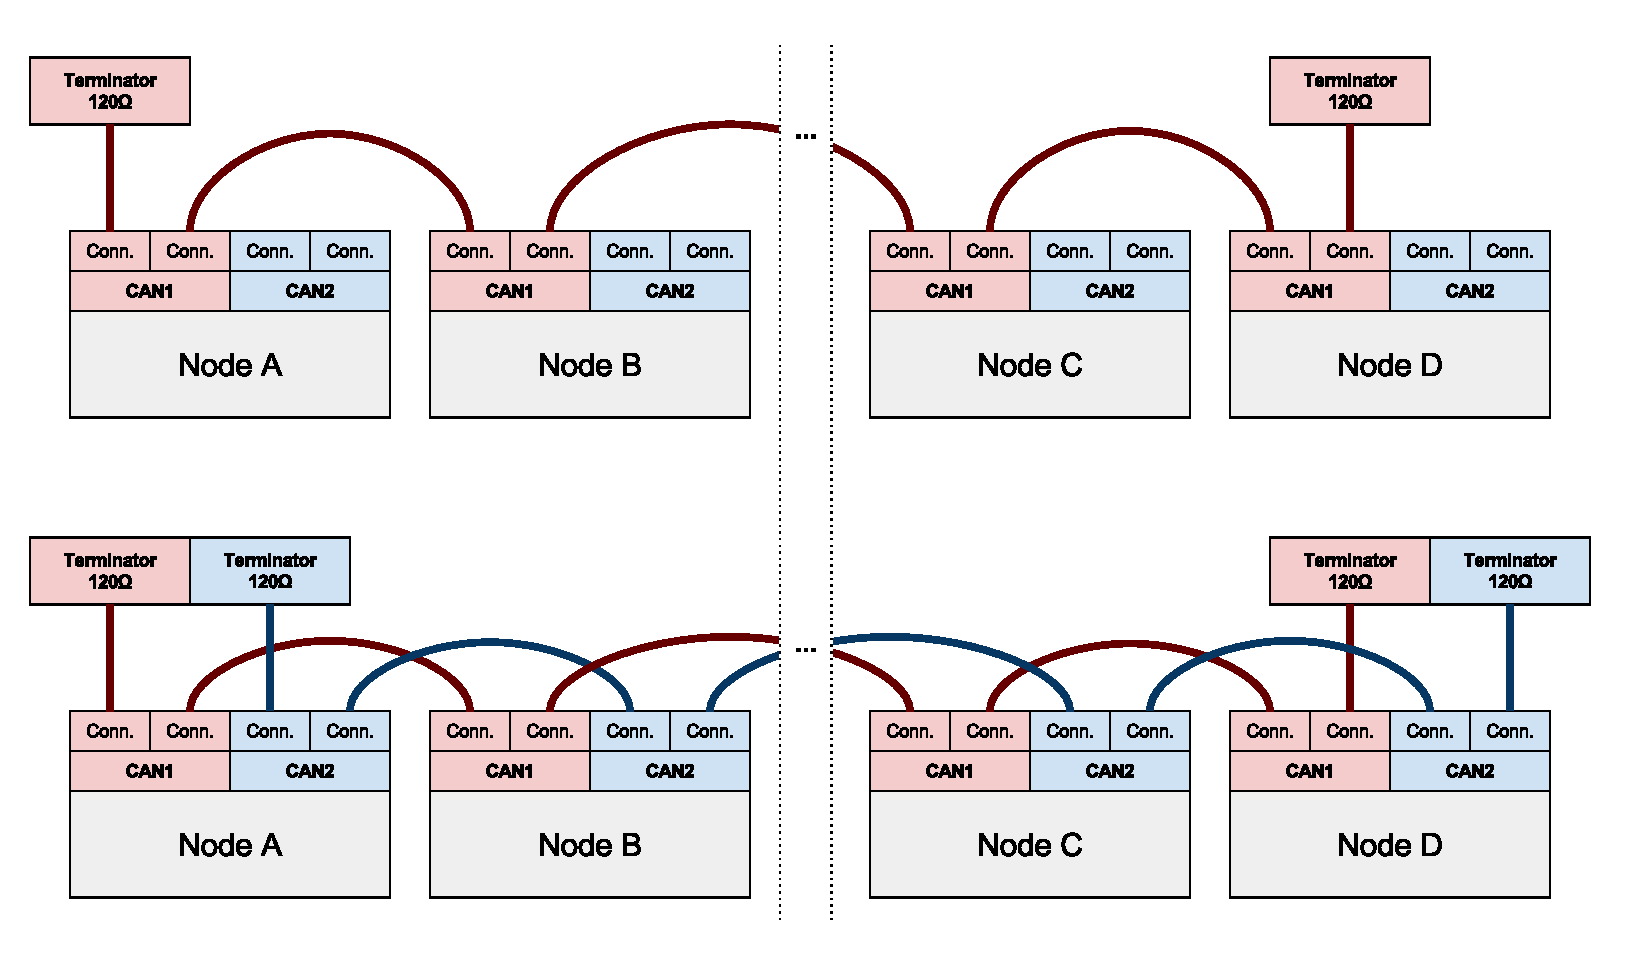
\includegraphics[width=\textwidth]{can_daisy_chain}
	\caption{Connection of CAN nodes in non-redundant and doubly redundant CAN bus configurations.
	\label{can_daisy_chain_non_redundant}}
\end{figure}

\section{Quality assurance}

Every manufactured Zubax Orel 20 undergoes an automated testing procedure that validates that
the device is functioning as designed.
The test log for every manufactured device is available on the web at
\url{https://device.zubax.com/device_info}.
This feature can be used to facilitate traceability of purchased devices and
provide additional safety assurances.

Besides testing, every manufactured device has a digital signature installed,
that can be used as a strong protection against unlicensed or counterfeit manufacturing.
Please refer to the dedicated documents or contact Zubax Robotics to find out
the specifics about digital signature verification.

\section{Enclosure}\label{sec:enclosure}

Zubax Orel 20 is intended for integration into the end system in the form of the bare PCB,
as this facilitates better heat dissipation, lower weight and tighter arrangement of components
in the end device, all of which are desirable properties in the target application domains.

Shall it be desired to provide additional mechanical protection for the device,
the plastic enclosure pictured on the figure \ref{enclosure} can be used.
Please contact your supplier for the ordering information;
alternatively, visit \url{https://github.com/Zubax/zubax_orel} to download
3D printable enclosure models suitable for in-house manufacturing.

\begin{figure}[hb]
	\centering
	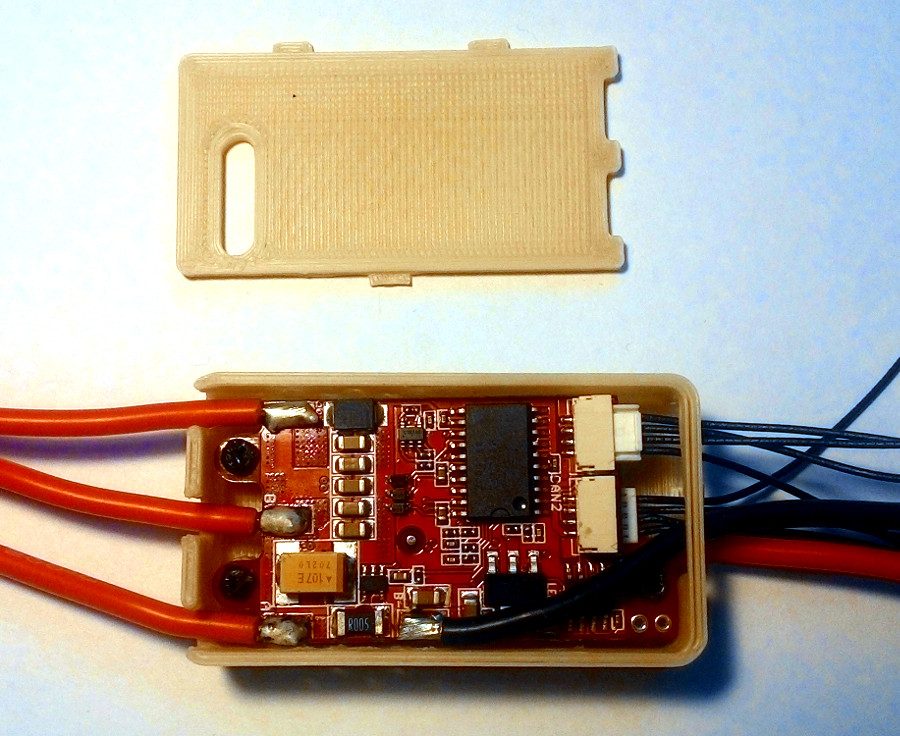
\includegraphics[width=0.45\textwidth]{enclosure-open}
	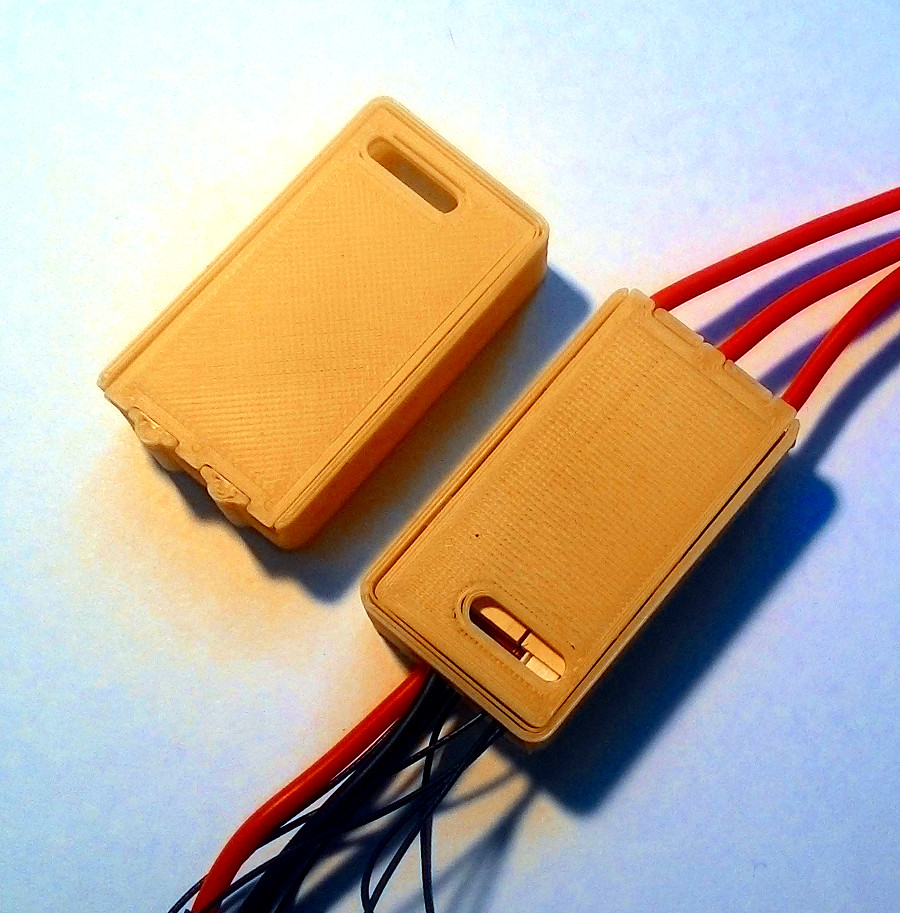
\includegraphics[width=0.45\textwidth]{enclosure-closed}
	\caption{Plastic enclosure.\label{enclosure}}
\end{figure}

\section{Accessories}

Zubax Orel 20 can be used with the following accessories:

\begin{itemize}
    \item Enclosure (suitable for 3D printing). See section \ref{sec:enclosure}.
    \item UAVCAN Micro patch cable.
    \item UAVCAN Micro adapter cables.
    \item UAVCAN Micro termination plug.
    \item Zubax DroneCode Debug Probe.
\end{itemize}

Please contact your supplier for ordering information.

\chapter{Characteristics}

\section{Absolute maximum ratings}

Subjecting the device to stresses beyond those specified in this section may cause
permanent damage to the device.
Proper operation of the device within the ranges specified in this section is not implied.

\begin{ZubaxSimpleTable}{Absolute maximum ratings}{|c X|c c|c|}
    Symbol            & Parameter                & Min  & Max & Unit \\
	$V_\text{inv}$    & Supply voltage           & -0.3 & 19  & V \\
	$T_\text{oper}$   & Operating temperature    & -50  & 125 & \degree{}C \\
	                  & UART/RCPWM input voltage & -0.3 & 7   & V\\
	                  & CAN H/L input voltage    & -4   & 16  & V\\
\end{ZubaxSimpleTable}

\section{Environmental conditions}

\begin{ZubaxSimpleTable}{Environmental conditions}{|c X|l|c c|c|}
    Symbol & Parameter & Note & Min & Max & Unit \\
	$T_\text{oper}$ & Operating temperature &                            & -40 & 105 & \degree{}C \\
	$T_\text{stor}$ & Storage temperature   &                            & -40 & 50  & \degree{}C \\
	$\phi_\text{oper}$ & Operating humidity & Condensation not permitted & 0   & 100 & \%RH\\
	$h_\text{oper}$ & Operating altitude    & Above mean sea level (MSL) &     & 10  & km\\
\end{ZubaxSimpleTable}

\section{Reliability}

\begin{ZubaxSimpleTable}{Reliability}{|c X|c|c|}
    Symbol & Parameter & Typ & Unit \\
	MTTF   & Mean time to failure & 100000 & hours \\
\end{ZubaxSimpleTable}

\section{Power characteristics}

\begin{ZubaxTableWrapper}{Power characteristics}
	\begin{ZubaxWrappedTable}{|c X|c c c|c|}
	    Symbol & Parameter & Min & Typ & Max & Unit \\
		$P$                 & Continuous power                    &      &      & 350  & W \\
		$P_\text{peak}$     & Peak power                          &      &      & 1000 & W \\
		$I_\text{inv}$      & Continuous DC current               &      &      & 20   & A \\
		$I_\text{inv-peak}$ & Peak DC current                     &      &      & 55   & A \\
		$I_\text{idle}$     & Idle current consumption            &      & 50   &      & mA \\
		$V_\text{inv}$      & Supply voltage\tnote{1}             & 9    & 14.8 & 18.5 & V \\
	    $V_\text{TVS}$      & TVS\tnote{2}\space{} circuit
	                          activation voltage                  & 19   &      & 21   & V \\
	    $P_\text{TVS}$      & TVS circuit maximum power
	                          dissipation                         &      & 1000 &      & W \\
	    $E_\text{TVS}$      & TVS circuit energy absorption
	                          capability\tnote{3}                 &      & 5    &      & J \\
		$\theta_\text{JA}$  & Junction-to-air thermal resistance  &      & 50   &      & K/W \\
	    $R_\text{DS-on}$    & FET drain-source on-state resistance&      & 1.6  & 1.9  & $\text{m}\Omega$ \\
	    $R_\text{phase}$    & Cumulative resistance of the
	                          inverter per phase                  &      & 5    &      & $\text{m}\Omega$ \\
	                        & Inverter temperature measurement
	                          error                               & -6   &      & +6   & \degree{}C \\
	                        & Inverter temperature measurement
	                          range                               & -55  &      & 125  & \degree{}C \\
	\end{ZubaxWrappedTable}
	\begin{tablenotes}
	    \item [1] Suitable battery packs per chemistry type:\\
	    \begin{ZubaxCompactTable}{|c c c|}
		    Chemistry         & Nominal cell voltage [V] & Cells in series [S]\\
		    $\text{LiCoO}_2$  & 3.7                      & \numrange{3}{4}\\
		    $\text{LiFePO}_4$ & 3.3                      & \numrange{4}{5}\\
		    $\text{NiCd}$, $\text{NiMH}$ & 1.2           & \numrange{10}{12}\\
		    $\text{Pb}$       & 2.0                      & \numrange{6}{8}\\
	    \end{ZubaxCompactTable}
	    
	    \item [2] Transient voltage suppression.

	    \item [3] At $T = 25\text{\degree{}C}$, non-repetitive.
	\end{tablenotes}
\end{ZubaxTableWrapper}

\subsection{Regenerative braking}

During regenerative braking, the device performs energy transfer from the motor to the power supply network.
If the self resistance of the power supply network is not sufficiently low,
the regenerative energy transfer may lead to increase of the supply voltage beyond
the safe operating limits.
This event will trigger activation of the transient voltage suppression (TVS) circuit,
which will absorb some of the excessive energy.
If the amount of recovered energy exceeds the absorption capabilities of the power supply
network and the TVS circuit, the device may incur fatal damage.

Generally, batteries are capable of absorbing the regenerated energy during braking without issues.
Problems may arise if the device is powered from a source that does not permit reverse currents,
such as laboratory power supplies.
In the latter case it is advised to install additional buffer capacitors to act as an energy buffer
during braking.

\subsection{Power connectors}

Zubax Orel 20 is equipped with bullet 3.5 mm power connectors.
Input power is provided via male connectors soldered on 100 mm long 16 AWG wires.
The motor phases are connected via female connectors soldered on 100 mm long 16 AWG wires.
Additional connection options are available upon request.

\section{Communication interfaces}

\subsection{CAN bus}

The device is equipped with doubly redundant CAN 2.0A/B interface.
Each CAN interface has two standard UAVCAN Micro connectors\footnote{Refer to
\url{http://uavcan.org} for more information on UAVCAN.}
joined in parallel.
The power rails of the connector pairs are not connected to the device's internal circuitry,
since Zubax Orel 20 does not consume or provide power to the CAN bus.

The device does not terminate the CAN bus internally.

CAN2 (the secondary CAN bus interface) can only be used in configurations with redundant CAN bus.
If the bus is not redundant, only CAN1 (the primary CAN bus interface) can be used.
Connectors of unused CAN bus interfaces should be left empty.

\begin{ZubaxSimpleTable}{CAN bus connectors pinout}{|c X X X[3]|}
	Pin no. & Type         & Name      & Comment \\
	1       & Power        & PWR       & Not connected to the device's circuits internally.\\
	2       & Input/Output & CAN H     & \\
	3       & Input/Output & CAN L     & \\
	4       & Ground       & GND       & \\
\end{ZubaxSimpleTable}

\begin{ZubaxTableWrapper}{Characteristics of CAN bus interfaces}
	\begin{ZubaxWrappedTable}{|c X|c c c|c|}
		Symbol  & Parameter                                 & Min  & Typ  & Max  & Unit \\
		        & Bit rate                                  & 20   &      & 1000 & Kbps \\
		        & Positive-going input threshold voltage    &      & 750  & 900  & mV \\
		        & Negative-going input threshold voltage    & 500  & 600  &      & mV \\
		        & Differential output voltage, dominant     & 1.5  & 2.0  & 3.0  & V \\
		        & Differential output voltage, recessive    & -120 & 0    & 12   & mV \\
		        & Bus power rail\tnote{1}\space{} voltage   & -10  &      & 10   & V \\
		        & Inter-connector current\tnote{1}          & -1 &  & 1    & A \\
		        & Connector resistance during device lifetime &    & 30   & 50   & $\text{m}\Omega$ \\
	\end{ZubaxWrappedTable}
	\begin{tablenotes}
	    \item [1] The limit is imposed by the PCB.
	\end{tablenotes}
\end{ZubaxTableWrapper}

\subsection{DroneCode debug port}

The device features a DroneCode debug port available via the standard
DroneCode Mini debug connector (DCD-M)\footnote{Refer to the DroneCode documentation
for more information on standard connectors and communication interfaces.}.
The DroneCode debug port provides access to the device's CLI\footnote{Command line interface.}
via UART, and to the RCPWM input which is shared with the UART RX line.

UART and RCPWM \emph{must not be used simultaneously}.
If RCPWM is activated, it is \emph{prohibited} to connect UART,
as that may cause unpredictable behavior of the RCPWM interface.

\begin{ZubaxSimpleTable}{DroneCode Mini debug connector pinout}{|c X X X|}
	Pin no. & Type         & Name                & Comment \\
	1       & Power        & TPWR                & 3.3 V power output \\
	2       & Output       & UART TX             & \\
	3       & Input        & UART RX \& RCPWM RX & Pulled down with a resistor\\
	4       & Input/Output & SWDIO               & Not for production use \\
	5       & Input        & SWDCLK              & Not for production use \\
	6       & Ground       & GND                 & \\
\end{ZubaxSimpleTable}

\begin{ZubaxSimpleTable}{DroneCode debug port characteristics}{|c X|c c c|c|}
	Symbol  & Parameter                                 & Min  & Typ  & Max  & Unit \\
			& Low-level input voltage                   & -0.3 & 0    & 1.6  & V\\
			& High-level input voltage                  & 2.1  & 3.3  & 5.5  & V\\
			& Low-level output voltage                  & 0    & 0    & 0.5  & V\\
			& High-level output voltage                 & 2.8  & 3.3  & 3.4  & V\\
			& Source/sink current via data pins         &      &      & 10   & mA\\
			& UART RX / RCPWM RX pull down resistance   & 15   & 20   & 25   & $\text{k}\Omega$\\
	$V_\text{DCDP}$ & Power rail output voltage         & 3.2  & 3.3  & 3.4  & V\\
	$I_\text{DCDP}$ & Power rail load capability        &      &      & 3    & mA\\
	        & Connector resistance during device lifetime &    & 20   & 40   & $\text{m}\Omega$\\
\end{ZubaxSimpleTable}

\subsection{RCPWM input}

The RCPWM interface has a dedicated connection point near the edge of the PCB,
suitable for soldering wires directly to it.
This connection point is connected directly to the UART RX / RCPWM RX pin,
and so it does not constitute an independent interface.
Same conditions and limitations apply.

\section{Indication}

Zubax Orel 20 is equipped with a single RGB LED indicator for purposes of status indication.
The LED is located on the bottom side near the edge of the PCB.

\section{Mechanical characteristics}

The drawing \ref{drawing} documents the basic mechanical characteristics of Zubax Orel 20,
such as the placement of connectors and mounting holes.

Both connectors of the primary CAN interface are located on the top side of the board.
They are explicitly marked as \verb|CAN1| on the PCB silkscreen.
Connectors of the secondary CAN interface are located on the bottom side of the board,
and marked \verb|CAN2|.

For reference, the red (positive) power supply wire is connected to the top side of the board.

\begin{figure}[!hbt]
	\centerline{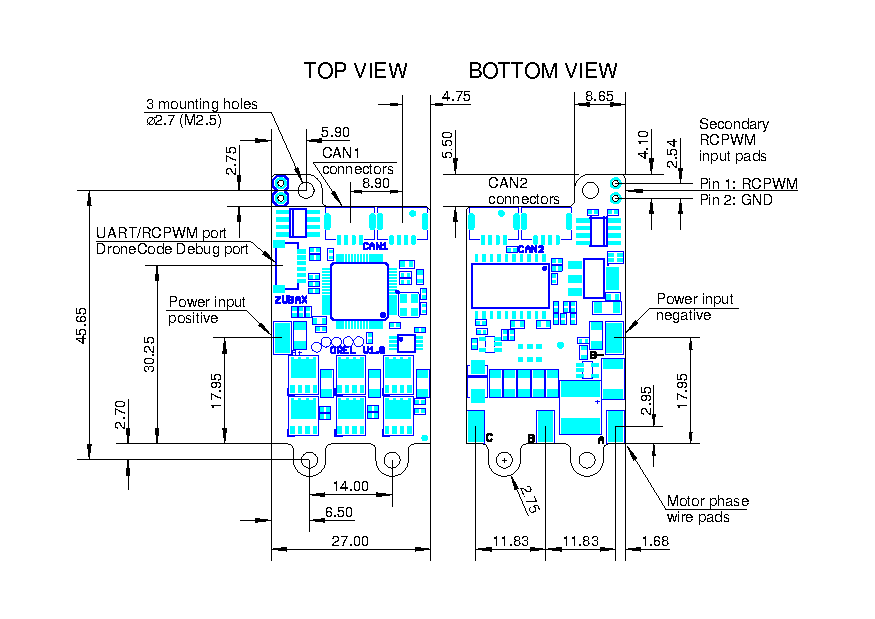
\includegraphics[width=1.1\textwidth]{drawing}}
	\caption{PCB drawing.\label{drawing}}
\end{figure}

\begin{ZubaxSimpleTable}{Mechanical characteristics}{|c X|l|c|c|}
    Symbol & Parameter & Note                          & Typ & Unit \\
	$m$    & Mass      & Power connectors not included & 10  & g \\
\end{ZubaxSimpleTable}

\end{document}
